% Drawing 154/04-10 -- folder 154, batch 04, archive page 80 (PDF page 81).
% Transcription: page de dessins en couleur, avec une seule légende : quatre disques au bord jaune ou vert, chacun traversé d'un arrangement de pseudo-droites orange (pleines ou pointillées) et d'un faisceau de lignes grises au crayon allant d'un point du bord au point antipodique. Sur le premier, une corde rouge épaisse suit le diamètre ; sur le deuxième et le troisième, deux arcs rouges épais forment un fuseau entre deux points antipodiques ; sur le quatrième, le fuseau s'est refermé en une ligne grise le long du diamètre. Des flèches mènent du premier aux trois autres, avec les légendes « $\frac12$ circuits autour de pts d'ordre $1$, $2$ » et « ou $0$ »
% Kind: four disks with arrangements, pencil sweeps and a spindle closing up. Method 2 (schematic redraw from the facsimile). Status: partial.
% Notes: Page of drawings in colour with one legend: four disks with yellow or green rims, each crossed by an orange arrangement (solid or dotted strands) and by a pencil sweep of grey lines from a point of the rim to the antipodal point. On the first a thick red chord follows the diameter; on the second and third two thick red arcs form a spindle between two antipodal points; on the fourth the spindle has closed up into a grey line along the diameter. Arrows lead from the first to the three others, with the legends « 1/2 circuits autour de pts d'ordre 1, 2 » and « ou 0 ». Disks, red chord and spindles placed from the page view; the orange arrangements (eight strands each, some dotted) and the grey sweeps are schematic.
% Coordinates: 1 unit = 1 mm = 1/100 of the crop width (bbox in page fractions: [0.157, 0.079, 0.846, 0.47]).
% Redrawn by Claude (claude-opus-5-5), issue #73, 2026-11-07; not checked by a human; not compiled (no TeX in the session).
% Rights: reproduces part of the work -- behind RENDER_TRANSCRIPTS, never published by itself.
\documentclass[tikz,border=3pt]{standalone}
\usepackage{amsmath,amssymb}
\usetikzlibrary{patterns,arrows.meta}
\tikzset{Or/.style={orange!90!black}, Ye/.style={yellow!80!orange}, Lg/.style={green!60!black!70}, Dg/.style={green!45!black}, Br/.style={brown!80!black}, Rd/.style={red!85!black}, Bl/.style={blue!70!black}, Gy/.style={black!40}, pencil/.style={black!45}, struck/.style={black!35}, mark/.style={circle,draw,inner sep=1.3pt}, pt/.style={circle,fill,inner sep=0.9pt}, opt/.style={circle,draw,fill=white,inner sep=1.1pt}}
\begin{document}
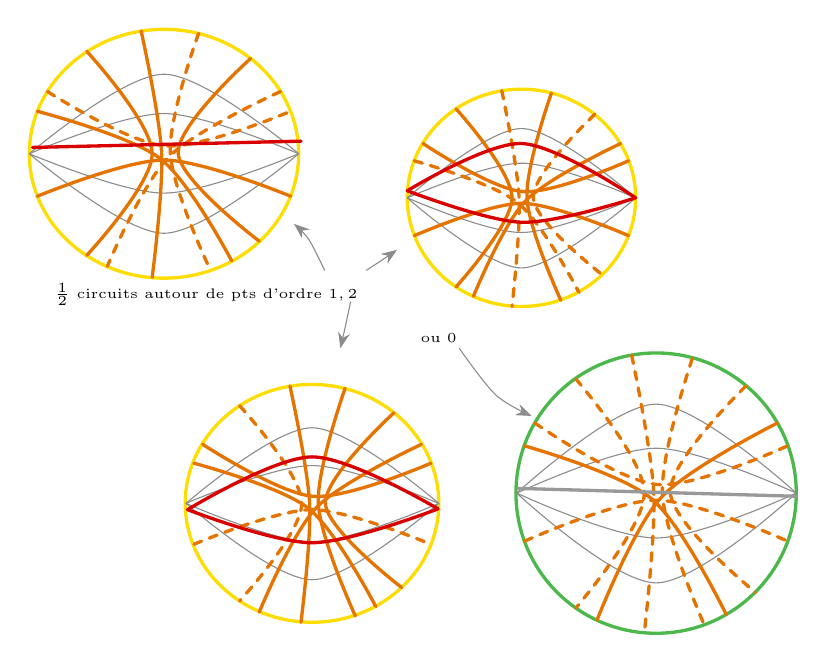
\begin{tikzpicture}[x=1mm,y=1mm,line cap=round,line join=round,font=\scriptsize]
\draw[Ye,very thick] (18.4,-17.4) ellipse[x radius=17.1, y radius=15.8];
\draw[pencil] plot[smooth, tension=0.55] coordinates {(1.3,-17.4) (18.4,-7.3) (35.5,-17.4)};
\draw[pencil] plot[smooth, tension=0.55] coordinates {(1.3,-17.4) (18.4,-12.3) (35.5,-17.4)};
\draw[pencil] plot[smooth, tension=0.55] coordinates {(1.3,-17.4) (18.4,-22.4) (35.5,-17.4)};
\draw[pencil] plot[smooth, tension=0.55] coordinates {(1.3,-17.4) (18.4,-27.5) (35.5,-17.4)};
\draw[Or,very thick] plot[smooth, tension=0.55] coordinates {(15.5,-1.8) (18.1,-17.4) (16.9,-33.1)};
\draw[Or,very thick,dashed] plot[smooth, tension=0.55] coordinates {(22.8,-2.1) (19.2,-17.3) (24.3,-32.2)};
\draw[Or,very thick] plot[smooth, tension=0.55] coordinates {(8.6,-4.4) (16.9,-17.4) (8.6,-30.3)};
\draw[Or,very thick] plot[smooth, tension=0.55] coordinates {(29.4,-5.3) (20.2,-17.3) (30.5,-28.5)};
\draw[Or,very thick,dashed] plot[smooth, tension=0.55] coordinates {(3.6,-9.5) (18.5,-16.4) (34.5,-12)};
\draw[Or,very thick] plot[smooth, tension=0.55] coordinates {(2.3,-22.8) (18.4,-18.2) (34.5,-22.8)};
\draw[Or,very thick,dashed] plot[smooth, tension=0.55] coordinates {(33.2,-9.5) (19,-17.8) (11.2,-31.7)};
\draw[Or,very thick] plot[smooth, tension=0.55] coordinates {(2.3,-12) (17.9,-18) (27,-31)};
\draw[Rd,very thick] (1.7,-16.6) -- (35.8,-15.8);
\draw[Ye,very thick] (63.8,-23) ellipse[x radius=14.5, y radius=13.8];
\draw[pencil] plot[smooth, tension=0.55] coordinates {(49.3,-23) (63.8,-14.2) (78.3,-23)};
\draw[pencil] plot[smooth, tension=0.55] coordinates {(49.3,-23) (63.8,-18.6) (78.3,-23)};
\draw[pencil] plot[smooth, tension=0.55] coordinates {(49.3,-23) (63.8,-27.4) (78.3,-23)};
\draw[pencil] plot[smooth, tension=0.55] coordinates {(49.3,-23) (63.8,-31.9) (78.3,-23)};
\draw[Or,very thick,dashed] plot[smooth, tension=0.55] coordinates {(61.3,-9.4) (63.5,-23) (62.6,-36.8)};
\draw[Or,very thick] plot[smooth, tension=0.55] coordinates {(67.6,-9.7) (64.5,-23) (68.8,-36)};
\draw[Or,very thick] plot[smooth, tension=0.55] coordinates {(55.5,-11.7) (62.6,-23) (55.5,-34.3)};
\draw[Or,very thick,dashed] plot[smooth, tension=0.55] coordinates {(73.1,-12.4) (65.3,-23) (74.1,-32.8)};
\draw[Or,very thick] plot[smooth, tension=0.55] coordinates {(51.3,-16.1) (63.9,-22.2) (77.4,-18.3)};
\draw[Or,very thick] plot[smooth, tension=0.55] coordinates {(50.2,-27.8) (63.8,-23.7) (77.4,-27.8)};
\draw[Or,very thick] plot[smooth, tension=0.55] coordinates {(76.4,-16.1) (64.3,-23.4) (57.7,-35.5)};
\draw[Or,very thick,dashed] plot[smooth, tension=0.55] coordinates {(50.2,-18.3) (63.3,-23.6) (71.1,-35)};
\draw[Rd,very thick] plot[smooth, tension=0.55] coordinates {(49.3,-22.1) (63.8,-16.1) (78.3,-23)};
\draw[Rd,very thick] plot[smooth, tension=0.55] coordinates {(49.3,-22.1) (63.8,-26.1) (78.3,-23)};
\draw[Ye,very thick] (37.2,-61.8) ellipse[x radius=16.1, y radius=15.1];
\draw[pencil] plot[smooth, tension=0.55] coordinates {(21.2,-61.8) (37.2,-52.2) (53.3,-61.8)};
\draw[pencil] plot[smooth, tension=0.55] coordinates {(21.2,-61.8) (37.2,-57) (53.3,-61.8)};
\draw[pencil] plot[smooth, tension=0.55] coordinates {(21.2,-61.8) (37.2,-66.7) (53.3,-61.8)};
\draw[pencil] plot[smooth, tension=0.55] coordinates {(21.2,-61.8) (37.2,-71.5) (53.3,-61.8)};
\draw[Or,very thick] plot[smooth, tension=0.55] coordinates {(34.4,-46.9) (36.9,-61.9) (35.8,-76.9)};
\draw[Or,very thick] plot[smooth, tension=0.55] coordinates {(41.4,-47.2) (38,-61.8) (42.7,-76.1)};
\draw[Or,very thick,dashed] plot[smooth, tension=0.55] coordinates {(28,-49.4) (35.9,-61.8) (28,-74.2)};
\draw[Or,very thick] plot[smooth, tension=0.55] coordinates {(47.6,-50.3) (38.9,-61.8) (48.6,-72.5)};
\draw[Or,very thick] plot[smooth, tension=0.55] coordinates {(23.3,-54.3) (37.3,-60.9) (52.3,-56.7)};
\draw[Or,very thick,dashed] plot[smooth, tension=0.55] coordinates {(22.2,-67) (37.2,-62.6) (52.3,-67)};
\draw[Or,very thick] plot[smooth, tension=0.55] coordinates {(51.1,-54.3) (37.8,-62.3) (30.5,-75.6)};
\draw[Or,very thick] plot[smooth, tension=0.55] coordinates {(22.2,-56.7) (36.7,-62.4) (45.3,-74.9)};
\draw[Rd,very thick] plot[smooth, tension=0.55] coordinates {(21.4,-62.6) (37.2,-55.9) (53.2,-62.5)};
\draw[Rd,very thick] plot[smooth, tension=0.55] coordinates {(21.4,-62.6) (37.2,-66.8) (53.2,-62.5)};
\draw[Lg,very thick] (80.9,-60.5) ellipse[x radius=17.8, y radius=17.8];
\draw[pencil] plot[smooth, tension=0.55] coordinates {(63.2,-60.5) (80.9,-49.2) (98.7,-60.5)};
\draw[pencil] plot[smooth, tension=0.55] coordinates {(63.2,-60.5) (80.9,-54.8) (98.7,-60.5)};
\draw[pencil] plot[smooth, tension=0.55] coordinates {(63.2,-60.5) (80.9,-66.2) (98.7,-60.5)};
\draw[pencil] plot[smooth, tension=0.55] coordinates {(63.2,-60.5) (80.9,-71.9) (98.7,-60.5)};
\draw[Or,very thick,dashed] plot[smooth, tension=0.55] coordinates {(77.8,-43) (80.6,-60.5) (79.4,-78.2)};
\draw[Or,very thick,dashed] plot[smooth, tension=0.55] coordinates {(85.5,-43.4) (81.7,-60.5) (87,-77.2)};
\draw[Or,very thick,dashed] plot[smooth, tension=0.55] coordinates {(70.7,-46) (79.4,-60.5) (70.7,-75.1)};
\draw[Or,very thick,dashed] plot[smooth, tension=0.55] coordinates {(92.3,-46.9) (82.7,-60.4) (93.5,-73.1)};
\draw[Or,very thick,dashed] plot[smooth, tension=0.55] coordinates {(65.5,-51.6) (81,-59.4) (97.6,-54.5)};
\draw[Or,very thick,dashed] plot[smooth, tension=0.55] coordinates {(64.2,-66.6) (80.9,-61.4) (97.6,-66.6)};
\draw[Or,very thick] plot[smooth, tension=0.55] coordinates {(96.3,-51.6) (81.5,-61.1) (73.4,-76.6)};
\draw[Or,very thick] plot[smooth, tension=0.55] coordinates {(64.2,-54.5) (80.3,-61.2) (89.8,-75.9)};
\draw[Gy,very thick] (63.4,-59.9) -- (98.7,-60.9);
\node[inner sep=1pt] at (23.7,-35.3) {\tiny $\frac12$ circuits autour de pts d'ordre $1,2$};
\node[inner sep=1pt] at (53.3,-40.8) {\tiny ou $0$};
\draw[pencil,-{Stealth[length=2mm]}] plot[smooth, tension=0.55] coordinates {(38.8,-32.2) (36.8,-28.3) (34.9,-26.3)};
\draw[pencil,-{Stealth[length=2mm]}] plot[smooth, tension=0.55] coordinates {(44.1,-32.2) (46.1,-30.9) (48,-29.6)};
\draw[pencil,-{Stealth[length=2mm]}] plot[smooth, tension=0.55] coordinates {(42.1,-36.2) (41.4,-39.5) (40.8,-42.1)};
\draw[pencil,-{Stealth[length=2mm]}] plot[smooth, tension=0.55] coordinates {(55.9,-42.1) (60.5,-48) (65.1,-50.7)};
\end{tikzpicture}
\end{document}
